\documentclass[../main.tex]{subfiles}

\allowdisplaybreaks

\begin{document}
\section{Bias-Variance and Model Selection}
\subsection{“No Free Lunch” Theorems}
In this section we will talk about a generic learner performance on different problems. We want to know if a given algorithm is better than the others in every case. The short answer is no, any two optimization algorithms are equivalent when their performance is averaged across all possible problems. In a more formal manner we can define $ACC_G(L)$ as the accuracy of L on unseen data and $\mathcal{F}$ as the set of all possible concept $y=f(x)$ (all possible problems).
\begin{theorem}[No Free Lunch theorem]
    $\forall L,$ $\frac{1}{|\mathcal{F}|} \sum_{\mathcal{F}} ACC_G(L) = \frac{1}{2}$, given any distribution $\mathcal{P}$ over x and training set size N.
\end{theorem}
\begin{corollary}
    For any two learner $L_1$ and $L_2$, if $\exists$ a learning problem s.t. $ACC_G(L_1)>ACC_G(L_2)$ then $\exists$ a learning problem s.t. $ACC_G(L_1)<ACC_G(L_2)$
\end{corollary}
In practice we are saying that it doesn't exist a perfect learning algorithm that performs well in every scenario. So every algorithm is "specialized" on a given learning task. No algorithm is universally better than another one.

\subsection{Bias-Variance trade-off}
To efficiently select the model complexity we want to analyze its error on unseen data.

\subsubsection{Bias-Variance decomposition}
The bias–variance decomposition is a way of analyzing a learning algorithm's expected generalization error with respect to a particular problem as a sum of three terms, the bias, variance, and a quantity called the irreducible error, resulting from noise in the problem itself.
Assume to have a dataset $\mathcal{D}$ with N samples taken from $t_i = f(x_i) + \epsilon$, where $E[\epsilon] = 0$ and $Var[\epsilon] = \sigma^2$
Our objective is to find a model $y(x)$ that approximate $f$ as well as possible on unseen data.
Let's consider the expected square error on an unseen sample x
\begin{align*}
    E[(t-y(x))^2] & = E[t^2 + y(x)^2 -2ty(x)]                                                                                     \\
                  & = E[t^2] + E[y(x)^2] - E[2ty(x)]                                                                              \\
                  & \text{We can substitute t with its true function }f(x)                                                        \\
                  & = E[t^2] \pm E[t]^2 + E[y(x)^2] \pm E[y(x)]^2 - f(x)E[2y(x)]                                                  \\
                  & = Var[t] + E[t]^2 + Var[y(x)] + E[y(x)]^2 - 2f(x)E[y(x)]                                                      \\
                  & = Var[t] + Var[y(x)] + E[t]^2 + E[y(x)]^2 - 2f(x)E[y(x)]                                                      \\
                  & = Var[t] + Var[y(x)] + (f(x) - E[y(x)])^2                                                                     \\
                  & = \underbrace{Var[t]}_{\sigma^2} + \underbrace{Var[y(x)]}_{\text{Variance}} + \underbrace{E[f(x) - y(x)]^2}_{
        \text{Bias}^2} \numberthis
\end{align*}
As we can see we have three sources of error
\begin{itemize}
    \item $\sigma^2$: This is the irreducible error. It generates directly from the problem.
    \item Variance: This is an error from sensitivity to small fluctuations in the training set. High variance can cause an algorithm to model the random noise in the training data, rather than the intended outputs (overfitting).
    \item Bias: this is an error from erroneous assumptions in the learning algorithm. High bias can cause an algorithm to miss the relevant relations between features and target outputs (underfitting).
\end{itemize}
It's worth mentioning that the expectation is performed over different realization of the training set D.
Let's see an example
\begin{center}
    \begin{tabular}{cc}
        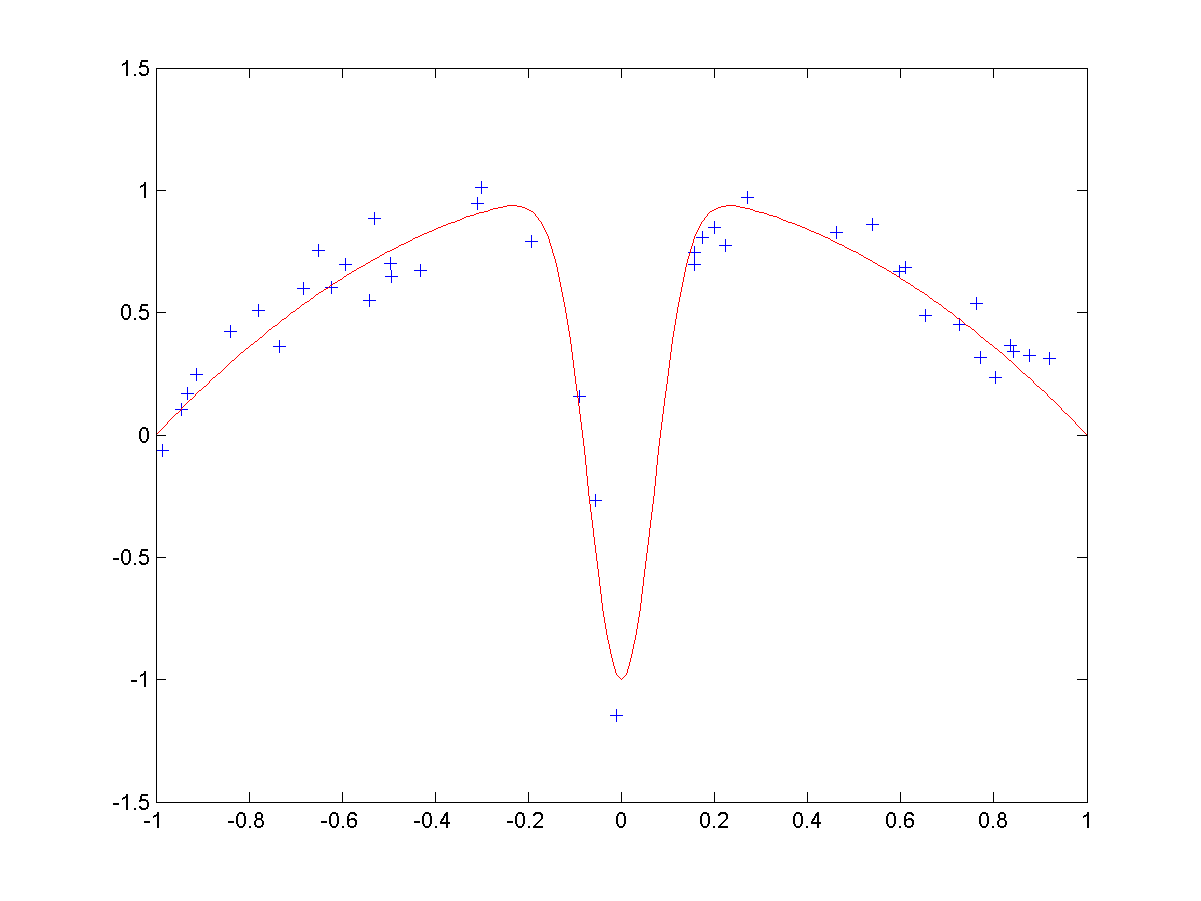
\includegraphics[width=70mm]{images/Test_function_and_noisy_data.png}        & 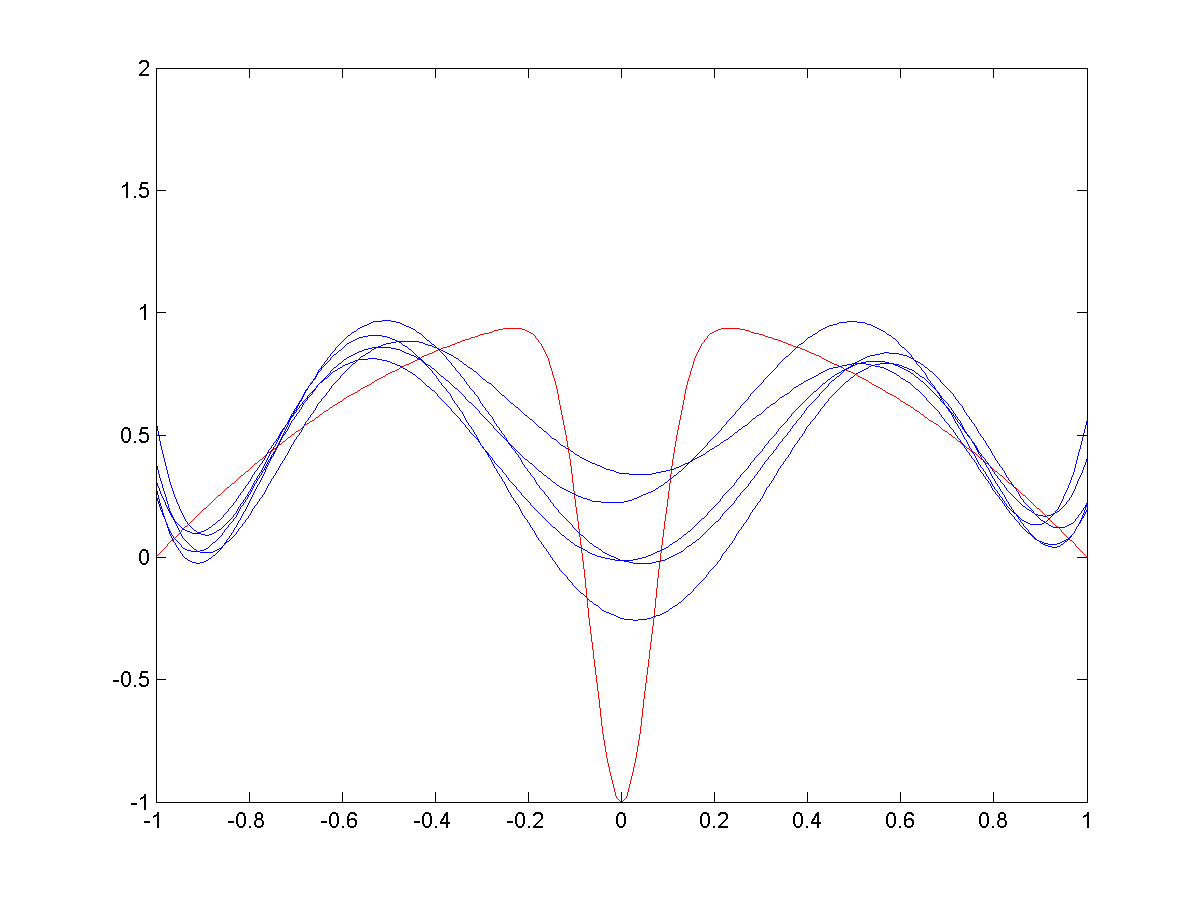
\includegraphics[width=70mm]{images/Radial_basis_function_fit,_spread=5.png}   \\
        (a)                                                                          & (b)                                                                            \\[6pt]
        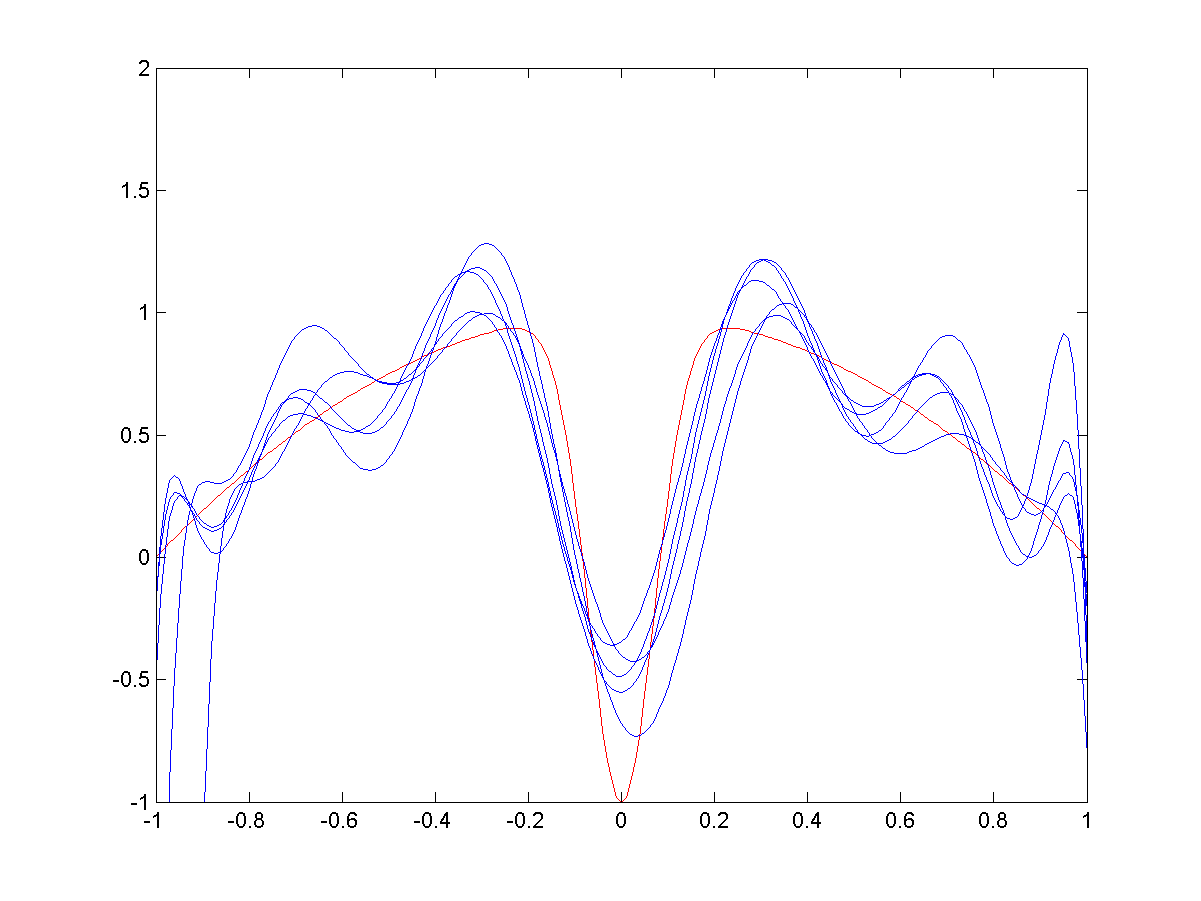
\includegraphics[width=70mm]{images/Radial_basis_function_fit,_spread=1.png} & 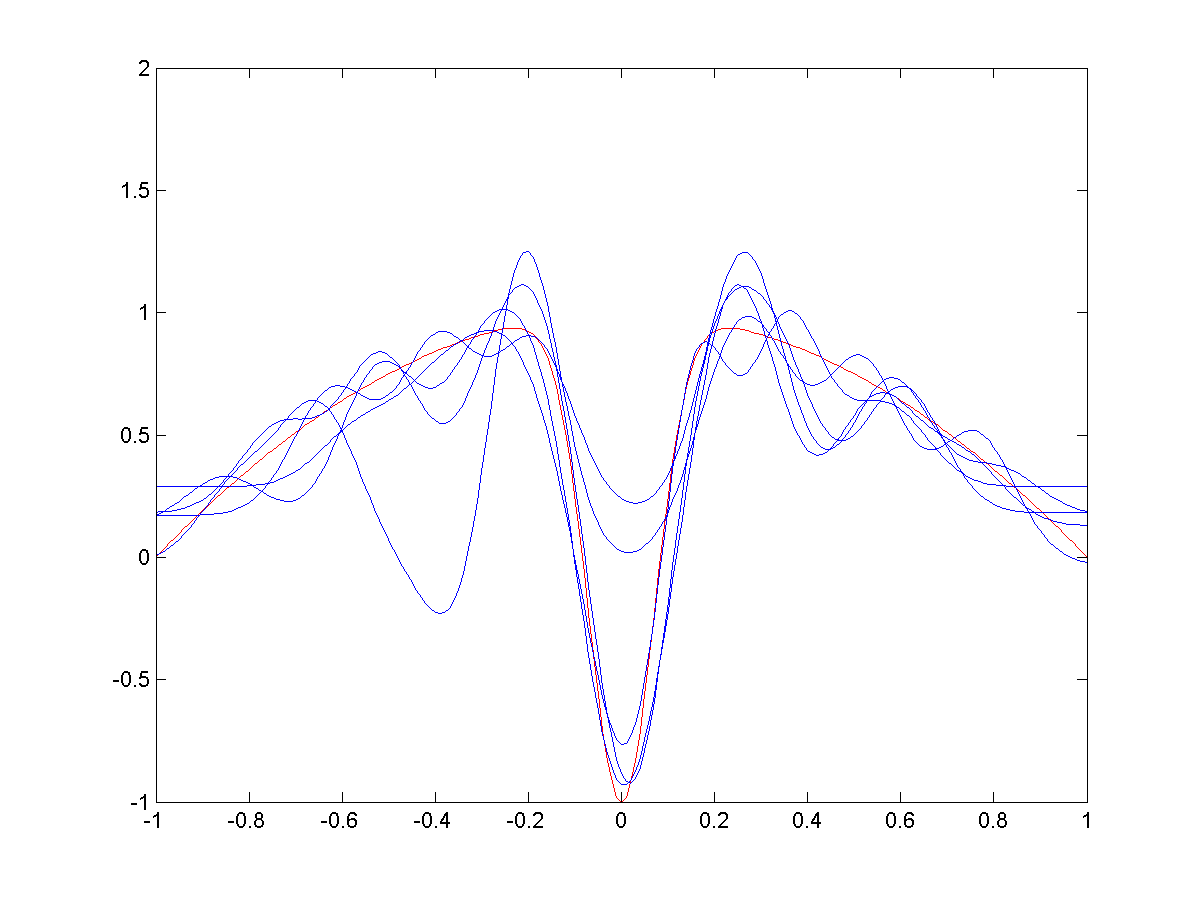
\includegraphics[width=70mm]{images/Radial_basis_function_fit,_spread=0.1.png} \\
        (c)                                                                          & (d)                                                                            \\[6pt]
    \end{tabular}
\end{center}
So let's take the dataset in figure(a) where the true function is the red line. For each case we take five different realization of the dataset and we estimate a model(blue line).
In figure(b) we have an underfitting situation because our model is too simple. We can observe that we have a big bias because the models don't fit on data. But the variance between the models is very low.
In figure(c) we have the right trade-off between bias and variance.
In figure(d) we have a very low bias because all the models estimate the dataset well, but the variance between the trials is very big. In this case we are overfitting the data.

\newpage
From what we have said, we can see how model complexity can affect the estimation error. Generally speaking the bias decreases with model complexity and variance increase with model complexity.

\begin{center}
    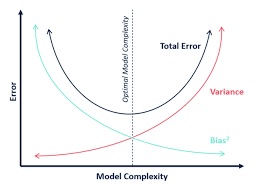
\includegraphics[scale=1.2]{images/Bias-Variance-tradeoff.png}
\end{center}
\paragraph{Example (K-NN)} In the case of K-Nearest Neighbor we can derive an explicit analytical expression of the expected squared prediction error
\begin{equation}
    E[(t-y(x))^2] = \sigma^2 + \frac{\sigma^2}{K} + \bigg( f(x) - \frac{1}{K}\sum_{i=1}^K f(x_i) \bigg)^2
\end{equation}
\begin{itemize}
    \item $\sigma^2$ is the irreducible error
    \item $\frac{\sigma^2}{K}$ is the variance term. It depends on the irreducible error and decreases as K increases
    \item $\bigg( \frac{1}{K}\sum_{i=1}^K f(x_i) \bigg)^2$ is the bias term. It depends on how rough the model space is. The rougher the space, the faster the bias term will increase as further away neighbors are brought into the estimates
\end{itemize}
\newpage
\subsubsection{Training-test error}
Given a data set $\mathcal{D}$ with N samples, we can split it in a training set and a test set.
To calculate the training error we have to choose a loss function(e.g. RSS).
We can distinguish between
\begin{itemize}
    \item Regression: $L_{train} = \frac{1}{N} \sum_{n=1}^N (t_n - y(x_n))^2$
    \item Classification: $L_train = \frac{1}{N} \sum_{n=1}^N (I(t_n \neq y(x_n)))$
\end{itemize}
The training error measures how close our model is to training data. As we can imagine, increasing model complexity decreases the training error. But we also know that passed a certain complexity the generalization capability of our model will be decrease. So training error is not a good estimator of our model performance because is monotonically decreasing with model complexity, so it is an optimistically biased estimate of prediction error.
Our objective is to estimate the true prediction error,
\begin{itemize}
    \item Regression: $L_{true} = \int (f(x) - y(x))^2 p(x)dx$
    \item Classification: $L_{true} = \int I(f(x) \neq y(x)) p(x)dx$
\end{itemize}
This is impossible to estimate directly because we would need the true model f(x). A good way to estimate the prediction error is through the test error.
\begin{equation}
    L_{test} = \frac{1}{N_{test}} \sum_{n=1}^{N_{test}} (t_n - y(x_n))^2
\end{equation}
The test error is calculated with the test set. It is very important to not mix the training set and the test set, in order to get an unbiased estimation of the prediction error.
We use the training set to estimate the model's parameters and the test set to estimate the prediction error.
\begin{center}
    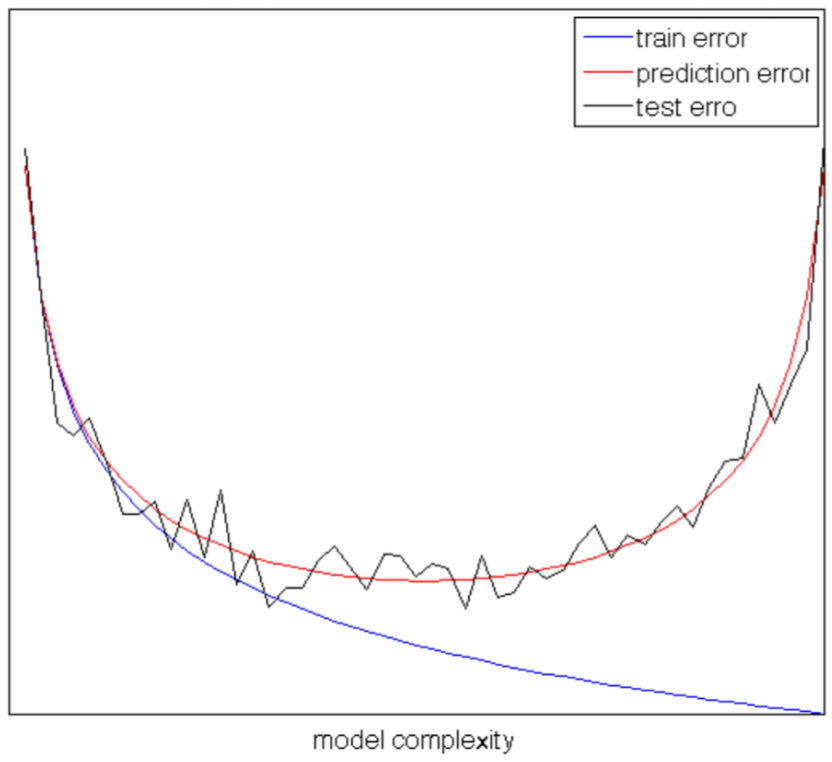
\includegraphics[scale=0.6]{images/prediction_error.PNG}
\end{center}

\newpage
\subsection{Model selection}
Model selection cover a key role in the performance of our model and can be performed in several ways.
Increasing the complexity of a model means to add dimensions to the input space. This could have really bad consequences.

\subsubsection{Curse of dimensionality} In ML we have the so called curse of dimensionality. It is related to the exponential increase in volume associated with adding extra dimensions to the input space. Working with high-dimensional data is difficult because the variance of the model becomes larger, we need more samples and computational power to counteract this phenomenon. So a common pitfall when we can't solve a learning problem is to add features to the input space. However the number of samples remain the same and so the importance of the old features decreases leading to worse performance. To have a better grasp of what can lead to an increasing search volume we can think of the following. Imagine the parameter space of a learning problem. Adding a feature will add a dimension in the parameter space. Let's imagine a uni-dimensional parameters space. Suppose we have two points on a line, 0 and 1. These two points are unit distance away from one another. Suppose we introduce a second axis, again distributed a unit distance away. Now we have two points, (0,0) and (1,1). But the distance between the points has grown to $\sqrt{2}$. If we iterate this process adding new dimension the two point will go further away. More formally, consider a p-dimensional hypercube with unit volume. Suppose that we have n points uniformally distributed inside the hypercube. Let r be the ratio of points inside the cube which are within some neighborhood. To capture an r-full of points in the data, we need to grow a cube which takes up r of the unit cube's volume. Since the length of an edge on the cube is simply 1, we have to find the cube edge $e$ so that $r=e^p$ is equal to the desired volume.
So expressed in terms of $e_p$, the edge length necessary to fill a p-hypercube is $e_p=r^{\frac{1}{p}}$. For example, to take 10\% of the point in a 2-dimensional space we have $e_2(0.1)=0.1^{\frac{1}{2}}=0.31$. Similarly, for a 10-dimension space we would have $e_{10}(0.1)=0.1^{\frac{1}{10}}=0.8$. To include 10\% of the data in a 10-dimensional space we need to take up to 80\% of the possible parameters values, in contrast in a 2-dimensional space we only need 31\%. The searching space grows exponentially.

\subsubsection{Feature selection}
Identifies a subset of input features that are most related to the output. We can use the following approach to select the best features.
\begin{enumerate}
    \item Let $\mathcal{M}_0$ be the null model which contains no input feature
    \item For $k=1,\dots,M$ (M different features)
          \begin{enumerate}
              \item Fit all $\binom{M}{k}$ models containing k features
              \item Pick the best model and call it $\mathcal{M}_k$. To define the \textit{best} model we need to define a metric.
          \end{enumerate}
    \item Select a single best model among $\mathcal{M}_0, \dots, \mathcal{M}_M$ using some criterion
\end{enumerate}
We can start from understanding how we can evaluate and select a single best model. Obviously we can't use training error, because the most complex model will perform "better", even though is overfitting. We would like to use the test error to evaluate which is the best model among a collection of models with different numbers of features. There are two approaches to estimate the test error
\begin{itemize}
    \item Direct estimation with a validation approach
    \item Making an adjustment to the training error to account for model complexity
\end{itemize}
\paragraph{Direct estimation}
So far we have divided the dataset into two subsets: training and test set. We do so to decouple the test data from the training phase in order to have an unbiased estimation of model performance. This decoupling must be preserved so \textbf{we can't use both training and test data to evaluate the various models and their features}. To have a fair evaluation we can introduce a new subset of data: \textbf{Validation set}.
\begin{itemize}
    \item \textbf{Training dataset}: The sample of data used to fit the model
    \item \textbf{Validation dataset}: The sample of data used to provide an unbiased evaluation of a model fit on the training dataset, while tuning model hyperparameters\footnotemark
    \item \textbf{Test dataset}: The samples of data used to provide an unbiased evaluation of the final model fit
\end{itemize}
\footnotetext{The hyperparameters are those parameters describing a model representation that cannot be learned by common optimization methods, but nonetheless affect the loss function. An example is the regularization parameter $\lambda$ in lasso}
In practice, the training set is used to learn the parameters, the validation set to tune the hyperparameter and the test set to evaluate the performance of our fit.
Validation set can't be use directly to estimate the error, because is used indirectly in the training phase. The solution is to use \textbf{cross validation}.
In practice we want to train the model on training set and evaluate it on the validation set. The novelty in the cross validation approach is that training and validation set are not fixed\footnotemark.\footnotetext{Every sample is used as training data and validation data in different phases of the learning process}
We can randomly divide the training data into k equal subsets: $\mathcal{D}_1, \dots, \mathcal{D}_k$. We learn k times the parameters producing k different models, each time excluding a different $\mathcal{D}_i$. Then we evaluate the performance of every model on the relative excluded set. To estimate the validation error we can calculate the average of every subset $\mathcal{D}_i$ error. Based on the parameter k we can have different type of cross validation error.
\paragraph{K-fold cross validation}
k-fold cross validation is the most used, because is a good trade-off between performance and accuracy. Usually we have $k \sim 10$\\
\begin{algorithm}[H]
    \SetAlgoLined
    \SetKwInOut{Input}{Input}
    \SetKwInOut{Output}{Output}
    \Output{Validation error $L_{k-fold}$}
    \Input{Data set $\mathcal{D}$ splitted in $\mathcal{D}_1, \dots, \mathcal{D}_k$
    }
    \For{$i\gets0$ \KwTo $k$}{
    Train model $y_{\mathcal{D} \setminus \mathcal{D}_i}$ on $\mathcal{D} \setminus \mathcal{D}_i$ \\
    $L_{\mathcal{D}_i} \leftarrow \frac{k}{N} \sum_{(x_n,t_n) \in \mathcal{D}_i} (t_n-y_{\mathcal{D} \setminus \mathcal{D}_i}(x_n))^2$
    }
    $L_{k-fold} \leftarrow \frac{1}{k} \sum_{i=1}^k L_{\mathcal{D}_i}$
    \caption{k-fold cross validation}
\end{algorithm}

\begin{center}
    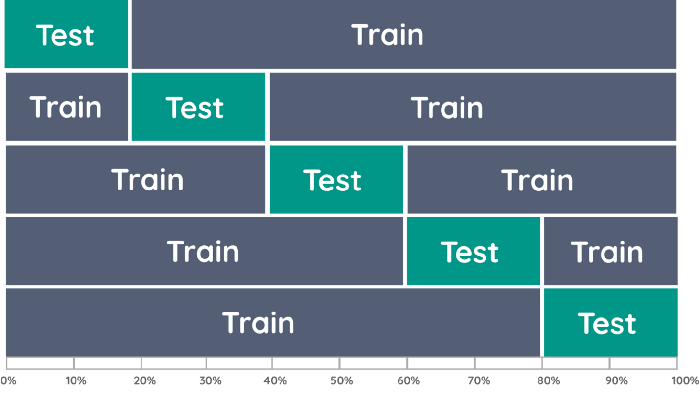
\includegraphics[height=40mm]{images/K-Fold.png}
\end{center}
It's worth mentioning that sometimes the validation partition is called test. Be aware that is not the same test set used ultimately to evaluate model performance.

\paragraph{LOO (Leave One Out)} In this case we consider at each iteration a validation set with only one sample. \\
\begin{algorithm}[H]
    \SetAlgoLined
    \SetKwInOut{Input}{Input}
    \SetKwInOut{Output}{Output}
    \Output{Validation error $L_{LOO}$}
    \Input{Data set $\mathcal{D}$ with N samples
    }
    \For{$i\gets0$ \KwTo $N$}{
    Train model $y_{\mathcal{D} \setminus \{n\}}$ on $\mathcal{D} \setminus \{n\}$ \\
    $L_{\{n\}} \leftarrow (t_n-y_{\mathcal{D} \setminus \{n\}}(x_n))^2$
    }
    $L_{LOO} \leftarrow \frac{1}{N} \sum_{n=1}^N L_{\{n\}}$
    \caption{LOO cross validation}
\end{algorithm}

\begin{center}
    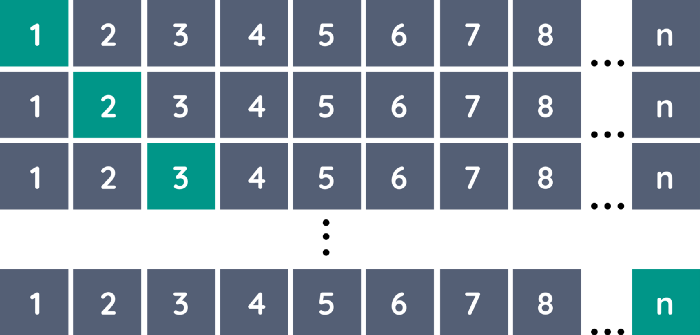
\includegraphics[height=40mm]{images/LOO.png}
\end{center}
To evaluate different input features set, we apply the cross validation for every model having those input features.
LOO is almost unbiased(pessimistically) as opposed to k-fold, but from a computational point of view k-fold is far better. For example, if we have 100.000 samples and each iteration of the algorithm takes 1 seconds, computing $L_{LOO}$ will take more than a full day. If you have to do it for every permutation of the input features it will take a very long time.

\paragraph{Adjustment techniques} This approach tries to account for model complexity when evaluating the training error. There are several way to do that
\begin{itemize}
    \item $C_p = \frac{1}{N} (RSS + 2d\Tilde{\sigma}^2)$ \\
          Where d is the number of parameters, $\Tilde{\sigma}^2$ is an estimate of the variance of the noise $\epsilon$
    \item $BIC = \frac{1}{N} (RSS + log(N)d\Tilde{\sigma}^2)$ \\
          We replaces $2d\Tilde{\sigma}^2$ of $C_p$ with $log(N)d\Tilde{\sigma}^2$. Since $log(N)>2$ when $N>7$, $BIC$ selects smaller models.
    \item $AIC = -2log(L) + 2d$ \\
          Where L is the maximized value of the likelihood function for the estimated model
    \item $AdjustedR^2 = 1- \frac{RSS/(N-d-1)}{TSS/(N-1)}$ \\
          where TSS is the total sum of squares. Differently from the other criteria, here a large value indicates a model with a small test error.
\end{itemize}

\newpage
\subsubsection{Regularization}
We have already seen regularization approaches applied to linear models like ridge regression and lasso. Such methods shrink the parameters towards zero. It may not be immediately obvious why such a constraint should improve the fit, but it turns out that shrinking coefficient estimates can significantly reduce the variance. A possible motivation could be that smaller parameters are less prone to produce fast changing output function, so they are less prone to overfitting because they can't interpolate directly all the samples. Regularization methods are very useful when we have limited dataset and a large number of features compared to the dataset size. To visualize the importance of choosing the correct regularization coefficient, we can consider the following example. We pick $N = 50$ samples from a given function and we try to fit it with a model with $45$ features. As a regression method we use ridge regression.
From the figure below we can see in action the bias-variance trade-off. When $\lambda$ gets bigger we obtain simpler models, so the variance is reduced and the bias gets bigger. We need to find the optimal $\lambda$ which minimizes the MSE. Cross-validation provides a simple way to tackle this problem. We choose a grid of $\lambda$ values, and compute the cross-validation error rate for each value of $\lambda$. We then select the tuning parameter value for which the cross-validation error is smallest. Finally, the model is re-fit using all of the available observations and the selected value of the tuning parameter.

\begin{center}
    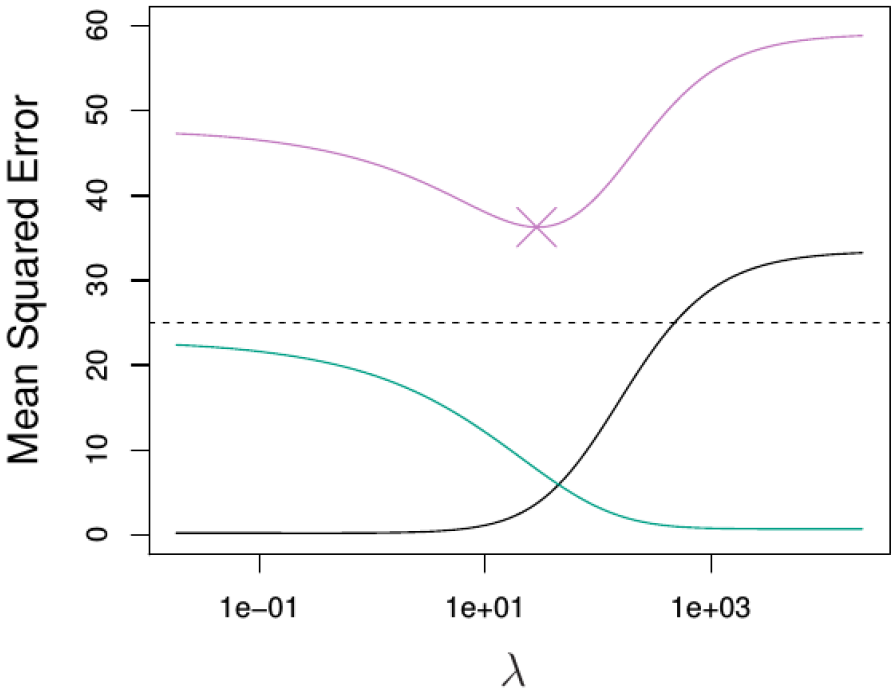
\includegraphics[width=90mm]{images/Lasso_MSE_Lambda.PNG} \\
    Black: squared bias, Green: variance, Purple: MSE, Dashed: minimum possible MSE, Purple cross: ridge regression model with minimum MSE
\end{center}

\subsubsection{Dimension reduction}
The approach we are going to present differs from the previous one because it doesn't operate directly on the original features. Dimension reduction methods transform the original features and then the model is learned on the transformed variables. It does so with an unsupervised learning approach. There are many techniques to perform dimensionality reduction,
\begin{itemize}
    \item PCA (Principal Component Analysis)
    \item ICA (Independent Component Analysis)
    \item Self-organizing Maps
    \item Autoencoders
    \item ...
\end{itemize}

\paragraph{PCA} The most used methodology is PCA. The idea is to find a new orthogonal base in the input space, which accounts for most of the input variance. In other word, we want to find a line such that when the data is projected onto that line, it has the maximum variance. Then we find a new line, orthogonal to the first one, that has maximum projected variance. We repeat this process until we have covered a certain percentage of input variance or we have reached a given number of dimensions(lines).
\begin{center}
    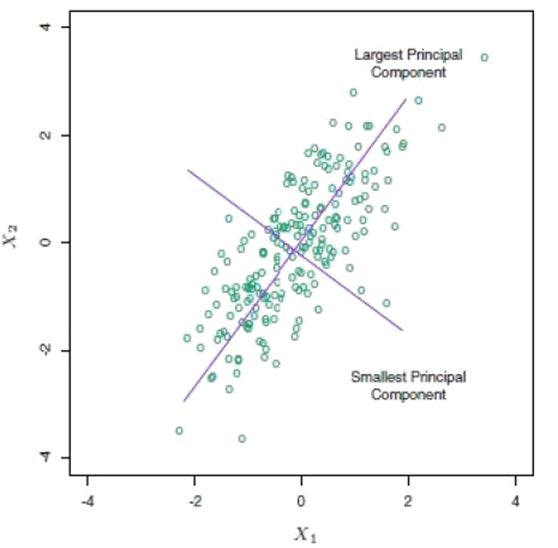
\includegraphics[width=90mm]{images/PCA.png} \\
\end{center}
In a more formal way, the complete process consists of,
\begin{enumerate}
    \item Compute the data mean $\overline{x} = \frac{1}{N} \sum_{n=1}^N x_n$ to later center the data on the origin
    \item Compute the covariance matrix $S = \frac{1}{N-1} \sum_{n=1}^N (x_n-\overline{x})(x_n-\overline{x})^T$
    \item Get the eigen values $\lambda_i$ and eigen vector $e_i$ of $S$
    \item Select the first k largest eigen values. The relative eigen vector are the PCA components. $\frac{\lambda_i}{\sum_i \lambda_i}$ is the percentage of variance captured by the $i^{th}$ principal component(PC)
\end{enumerate}
Once we have found the new PCs, we can project the data onto the new orthogonal base $E_k = \begin{bmatrix} e_1 & \dots & e_k \end{bmatrix}$ $[M \times k]$.
\begin{equation}
    X'=XE_k, \quad [N \times k]
\end{equation}

\begin{center}
    \begin{tabular}{c}
        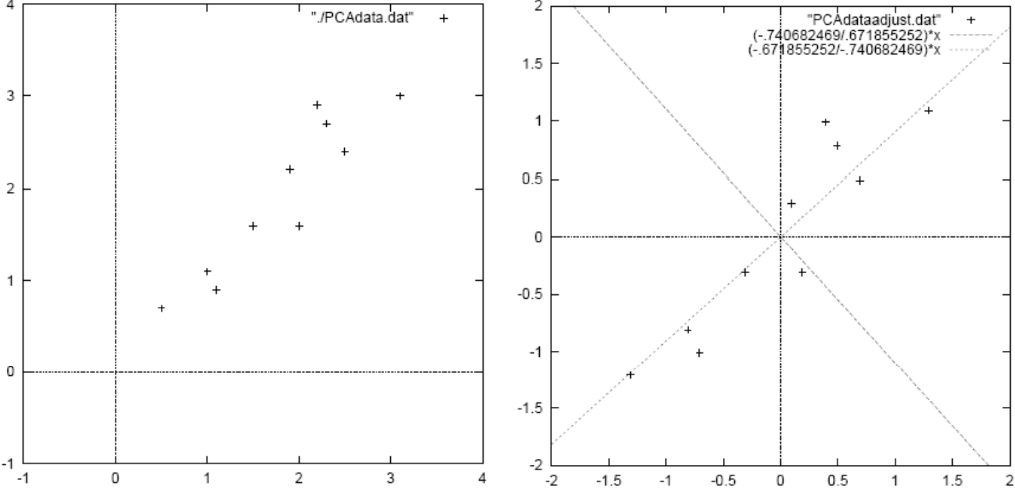
\includegraphics[width=140mm]{images/PAC_1.PNG}                                                    \\
        Left: Original data, Right: Mean centered data with PCs overlayed                                  \\[6pt]
        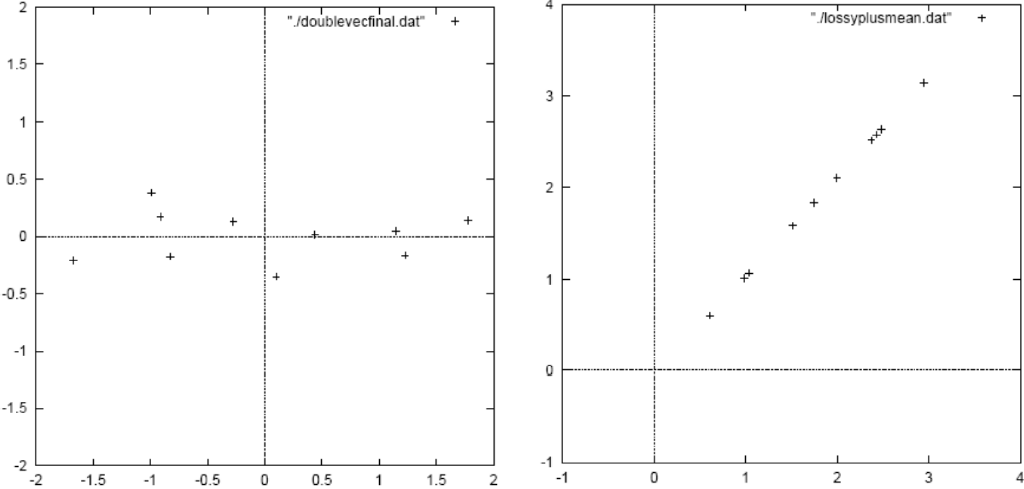
\includegraphics[width=140mm]{images/PAC_2.PNG}                                                    \\
        Left: Original data projected into full PC space, Right: Original data reconstructed with first PC \\[6pt]
    \end{tabular}
\end{center}

PCA is very useful to reduce computational complexity. In supervised learning reducing the number of dimension leads to smaller hypothesis space resulting in models that are less prone to overfitting. PCA can be seen as a noise reduction method.
This technique have some defects,
\begin{itemize}
    \item Fails when data consists of multiple cluster
    \item Directions of greatest variance may not be most informative
    \item Computational problems with many dimensions
    \item PCA computes linear combination of features, but data often lies on a nonlinear manifold
\end{itemize}

\subsection{Model Ensembles}
The methods seen so far can reduce bias by increasing variance or vice versa. But there's a class of technique that can reduce variance or bias only.
To decrease the variance without increasing the bias we can use \textbf{bagging}.
To decrease the bias without increasing the variance we can use \textbf{boosting}.
Bagging and Boosting are meta-algorithms. Their basic idea is to learn several models and combine them, instead of learning only one model. Typically they greatly improve accuracy.

\subsubsection{Bagging}
As we have said before bagging reduces the variance. We do so by averaging multiple models together. We know that
\begin{equation}
    Var[\Bar{X}] = \frac{Var[X]}{N}
\end{equation}
In order to be able to apply this method we need to find a way to generate multiple models from one dataset. To do so we use bootstrap.
This statistical technique consists in generating samples of size B (called bootstrap samples) from an initial dataset of size N by randomly drawing with replacement B observations.
\begin{center}
    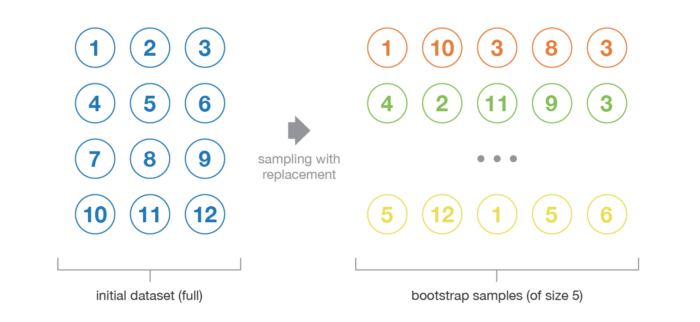
\includegraphics[width=110mm]{images/bootstrap.png}
\end{center}
After boostraping we train a model for each bootstrap sample. In the prediction phase, in case of classification the result will be the majority vote on the classification results of every model, and for regression will be the average of the predicted values estimated by every model. Bagging improves performance for unstable learners which vary significantly with small changes in the data set. In practice we want to average multiple overfitting model. From what we have studied before, an overfitting model has low bias and high variance. By combining different model we reduce the variance maintaining the low bias. In practice bagging almost always helps.

\subsubsection{Boosting}
The aim of boosting is to reduce the bias. It achieve so by sequentially train weak learners\footnotemark. Now you are wondering, what the fuck means sequentially.
Sequentially means that we train a model based on the prediction of the previous.
The steps to perform boosting are the following,
\begin{enumerate}
    \item Give an equal weight to all training samples
    \item Train a weak model on the training set
    \item Compute the error of the model on the training set
    \item For each training samples increase its weight if the model predicted wrong that sample. Doing so we obtain a new training set.
    \item Iterate the training on the new training set, error computation and samples re-weighting until we are satisfied by the result
\end{enumerate}
The final prediction is the weighted prediction of every weak learner. In practice we are combining a set of sequential underfitting model. Doing so, we have low variance and the bias is improved by combining the weak learner to form a strong learner.
On average, boosting helps more than bagging, but it is also more common for boosting to hurt performance.
\footnotetext{A weak learner is a learner that has a slightly better performance
    than chance prediction on any training set}

\newpage

\end{document}
